% Option 2:
% not finished, it is missing the results together

\section{Coupled simulations}

This section sets the road-map for conducting neutronics and thermal-fluids coupled simulations of prismatic HTGRs in Moltres.

\subsection{Discussion}
\label{sec:discuss}

This section analyzes Moltres' flaws at conducting prismatic HTGR coupled simulations.
% Describe moltres heterogenous capabilities as an MSR solver
Moltres' initial development targeted MSRs, allowing it to rely on heterogeneous diffusion calculations.
In a heterogeneous solver, each mesh node holds the information of each variable.
In an MSR simulation, Moltres defines the neutron flux and the temperature on each node.
Each node uses its temperature to compute the thermal feedback on the neutron flux.

% Moltres should use average temperatures
As discussed in Chapter \ref{ch:neutronics}, in a prismatic HTGR simulation, the neutronics calculation requires an assembly-level homogenization of the group constants.
Because of the homogenization, a mesh node holds the group constants' combined information from the different materials in the assembly --- only the fuel and the moderator as the coolant does not contribute considerably.
As the fuel group constants depended on the fuel temperature, and the moderator group constants depended on the moderator temperature, the thermal feedback depends on both temperatures.
Hence, a mesh node should hold both temperatures.

Moltres uses a heterogeneous thermal-fluid model to solve the temperature in the reactor.
The problem with using a heterogeneous model is that each node only holds the temperature's value in that particular material.
A coolant node holds the coolant temperature information and computes the thermal feedback with such information instead of the moderator and fuel temperature.
For this reason, Moltres should use the average assembly-level fuel and moderator temperatures instead of the point-wise temperature to compute the thermal feedback.

% Moltres should differentiate Tmod and Tfuel
One possible strategy is to homogenize the fuel and the moderator into one material.
Such homogenization assumes that both the moderator and fuel are in thermal equilibrium, and therefore have the same temperature.
Consequently, the model does not differentiate the fuel temperature from the moderator temperature.
However, a coupling model cannot correctly calculate the thermal feedback if it does not differentiate between the moderator and the fuel temperatures \cite{damian_vhtr_2008}.

We denominate this issue as the 'homogenization dilemma.'
To correctly compute neutronics, the diffusion solver must use homogenized parameters which depend on both moderator and fuel temperatures.
Simultaneously, to accurately calculate the thermal feedback, a mesh node should differentiate the moderator temperature from the fuel temperature, which require a heterogeneous calculation in the thermal-fluids model.
A thermal-fluid heterogeneous calculation is still valid, but the thermal feedback should use fuel and moderator average temperatures instead.
Next section develops a model that relies on this strategy.

\subsection{OECD/NEA MHTGR-350 MW Benchmark: Phase I Exercise 3}
\label{sec:ph1ex3}

% description of the exercise
This section conducted Phase I Exercise 3 of the benchmark with Moltres/MOOSE.
Exercise 3 combines all the data from the first two exercises, in which the participants need to determine a coupled neutronic and thermal-fluids solution.
The exercise requires the reporting of the same parameters reported in Exercises 1 and 2 combined.
The benchmark specifies the group constants necessary to conduct the exercise.
The group constants depend on four state parameters: moderator and fuel temperature and xenon-135 and hydrogen concentration.
In addition to these data, the benchmark provides fluence maps to determine the thermal conductivity of graphite.

Two sub-cases compose Exercise 3:
\begin{itemize}
  \item Exercise 3a: Same thermal-fluids problem definition from Exercise 2c. This exercise prescribes the bypass flow distribution and the thermo-physical properties depend on different simulation parameters.
  \item Exercise 3b: Same thermal-fluids problem definition from Exercise 2d. This exercise solves the bypass flow distribution through the explicit modeling of the bypass gaps. The thermo-physical properties depend on different simulation parameters.
\end{itemize}

% initial coupling: description of what I've done
Section \ref{sec:ph1ex2} solved the thermal-fluids standalone problem using a global and a sub-channel model.
Those simulations required running two separate input files, where the output of the global model served as an input to the sub-channel model.
Exercise 3 requires modeling the temperature feedback.
Using Section \ref{sec:ph1ex2} approach for the temperature feedback would require the fully-coupled simulation of both input files.
However, MOOSE framework does not have the capability to couple these specific problem input files.
To solve Exercise 3, we created a different model that homogenizes the fuel and moderator materials.
The solution did not differentiate between moderator and fuel, thus requiring the simulation of only the global model.

% describe the model
Figure \ref{fig:coupled-mesh} presents the model geometry.
The model includes 28 fuel and 29 coolant rings.
We calculated the radii of the rings by preserving the assemblies' and the coolant volume.
The coolant ring pitch is the coolant channel pitch in a fuel assembly.
Exercise 3a requires using material properties from Exercise 2c.
The simplified model used the material properties from Exercise 2a, as shown in Table \ref{tab:th-ex2a}.
The benchmark prescribes the group constants of 232 regions in the reactor.
Table \ref{tab:coupled-rz} shows what benchmark sub-domains integrate each model region.
The model did not include the control rod region (sub-domain 232).
The simulations used a three energy-group structure.
Table \ref{tab:coupled-eg} indicates what benchmark group numbers integrate each model group.
Conducting this exercise required the development of a tool to translate the benchmark group constants to Moltres format.
The tool was responsible for homogenizing and collapsing the group constants as well.
The problem assumed the same boundary conditions from Section \ref{sec:ph1ex2}.

Because Moltres can decouple the neutronics from the thermal-fluid effects, for the sake of comparison, we conducted the exercise with and without thermal feedback.
The calculations without thermal feedback assumed the group constants at 550 $^{\circ}$C.
The thermal feedback calculations used two strategies: one uses the point-wise temperature, and the second the average temperature to compute the feedback.
Figure \ref{fig:coupled-results-flux} and \ref{fig:coupled-results-th} display the results on two arbitrary located lines across the core.

The thermal feedback affects the flux, which consequently affects the thermal-fluids.
The axial flux peak moves towards the reactor top, where the temperatures are lower than the bottom.
Thus, the heat production shifts towards the reactor top, and the temperatures near the reactor outlet decrease.
The radial flux does not change considerably, hence the temperature profile does not change much either.
The thermal feedback moves the radial temperature profile up because of the heat production shift towards the top.

\begin{figure}[htbp!]
  \centering
  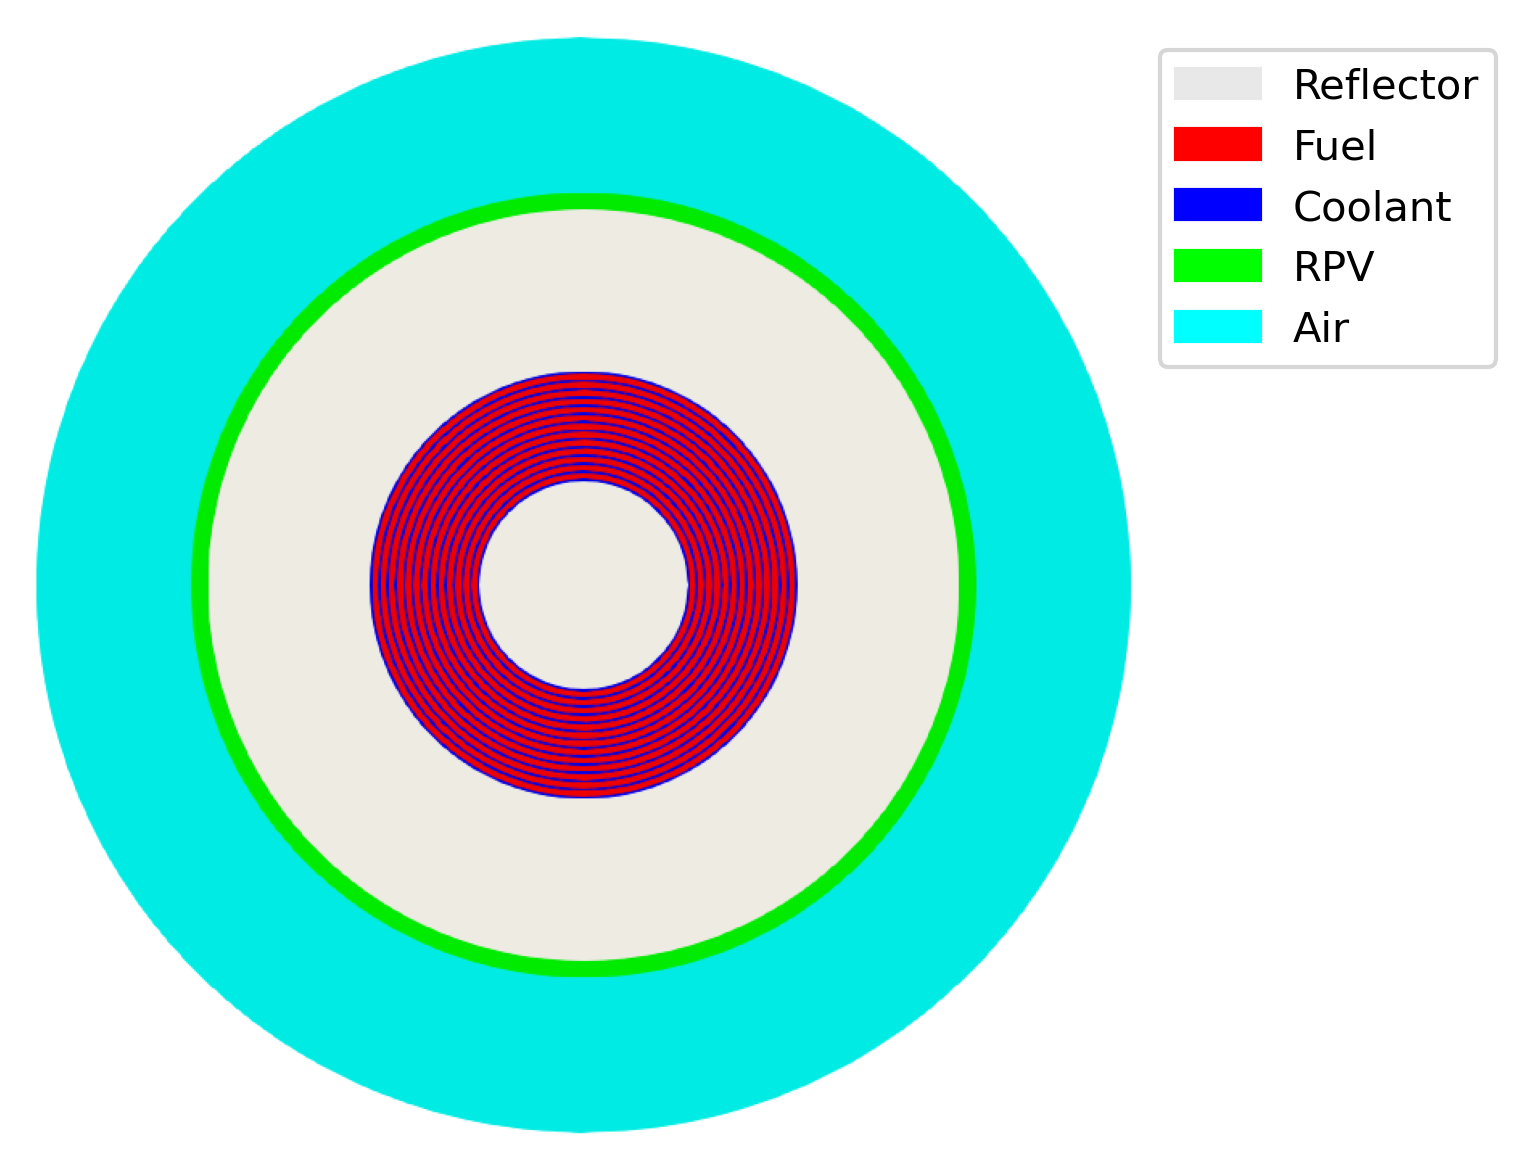
\includegraphics[width=0.45\linewidth]{figures-thermal/ex3-mesh}
  \hfill
  \caption{Model geometry.}
  \label{fig:coupled-mesh}
\end{figure}

\begin{table}[htbp!]
\centering
      \caption{Homogenization scheme.}
      \label{tab:coupled-rz}
    \begin{tabular}{l c}
  \toprule
  Model homogenized region & Benchmark sub-domains \\
  \midrule
  Fuel               & 1-220   \\
  Bottom reflector   & 221-224 \\
  Top reflector      & 228-231 \\
  Inner reflector    & 225     \\
  Outer reflector    & 226-227 \\
  \bottomrule
  \end{tabular}
\end{table}

\begin{table}[htbp!]
\centering
      \caption{Energy group condensation scheme.}
      \label{tab:coupled-eg}
    \begin{tabular}{c c}
  \toprule
  Model group number & Benchmark group number \\
  \midrule
  1 & 1-4   \\
  2 & 5-15  \\
  3 & 16-26 \\
  \bottomrule
  \end{tabular}
\end{table}

\begin{figure}[htbp!]
  \centering
    \subfloat[Axial flux over the line at r=85 cm.]{
        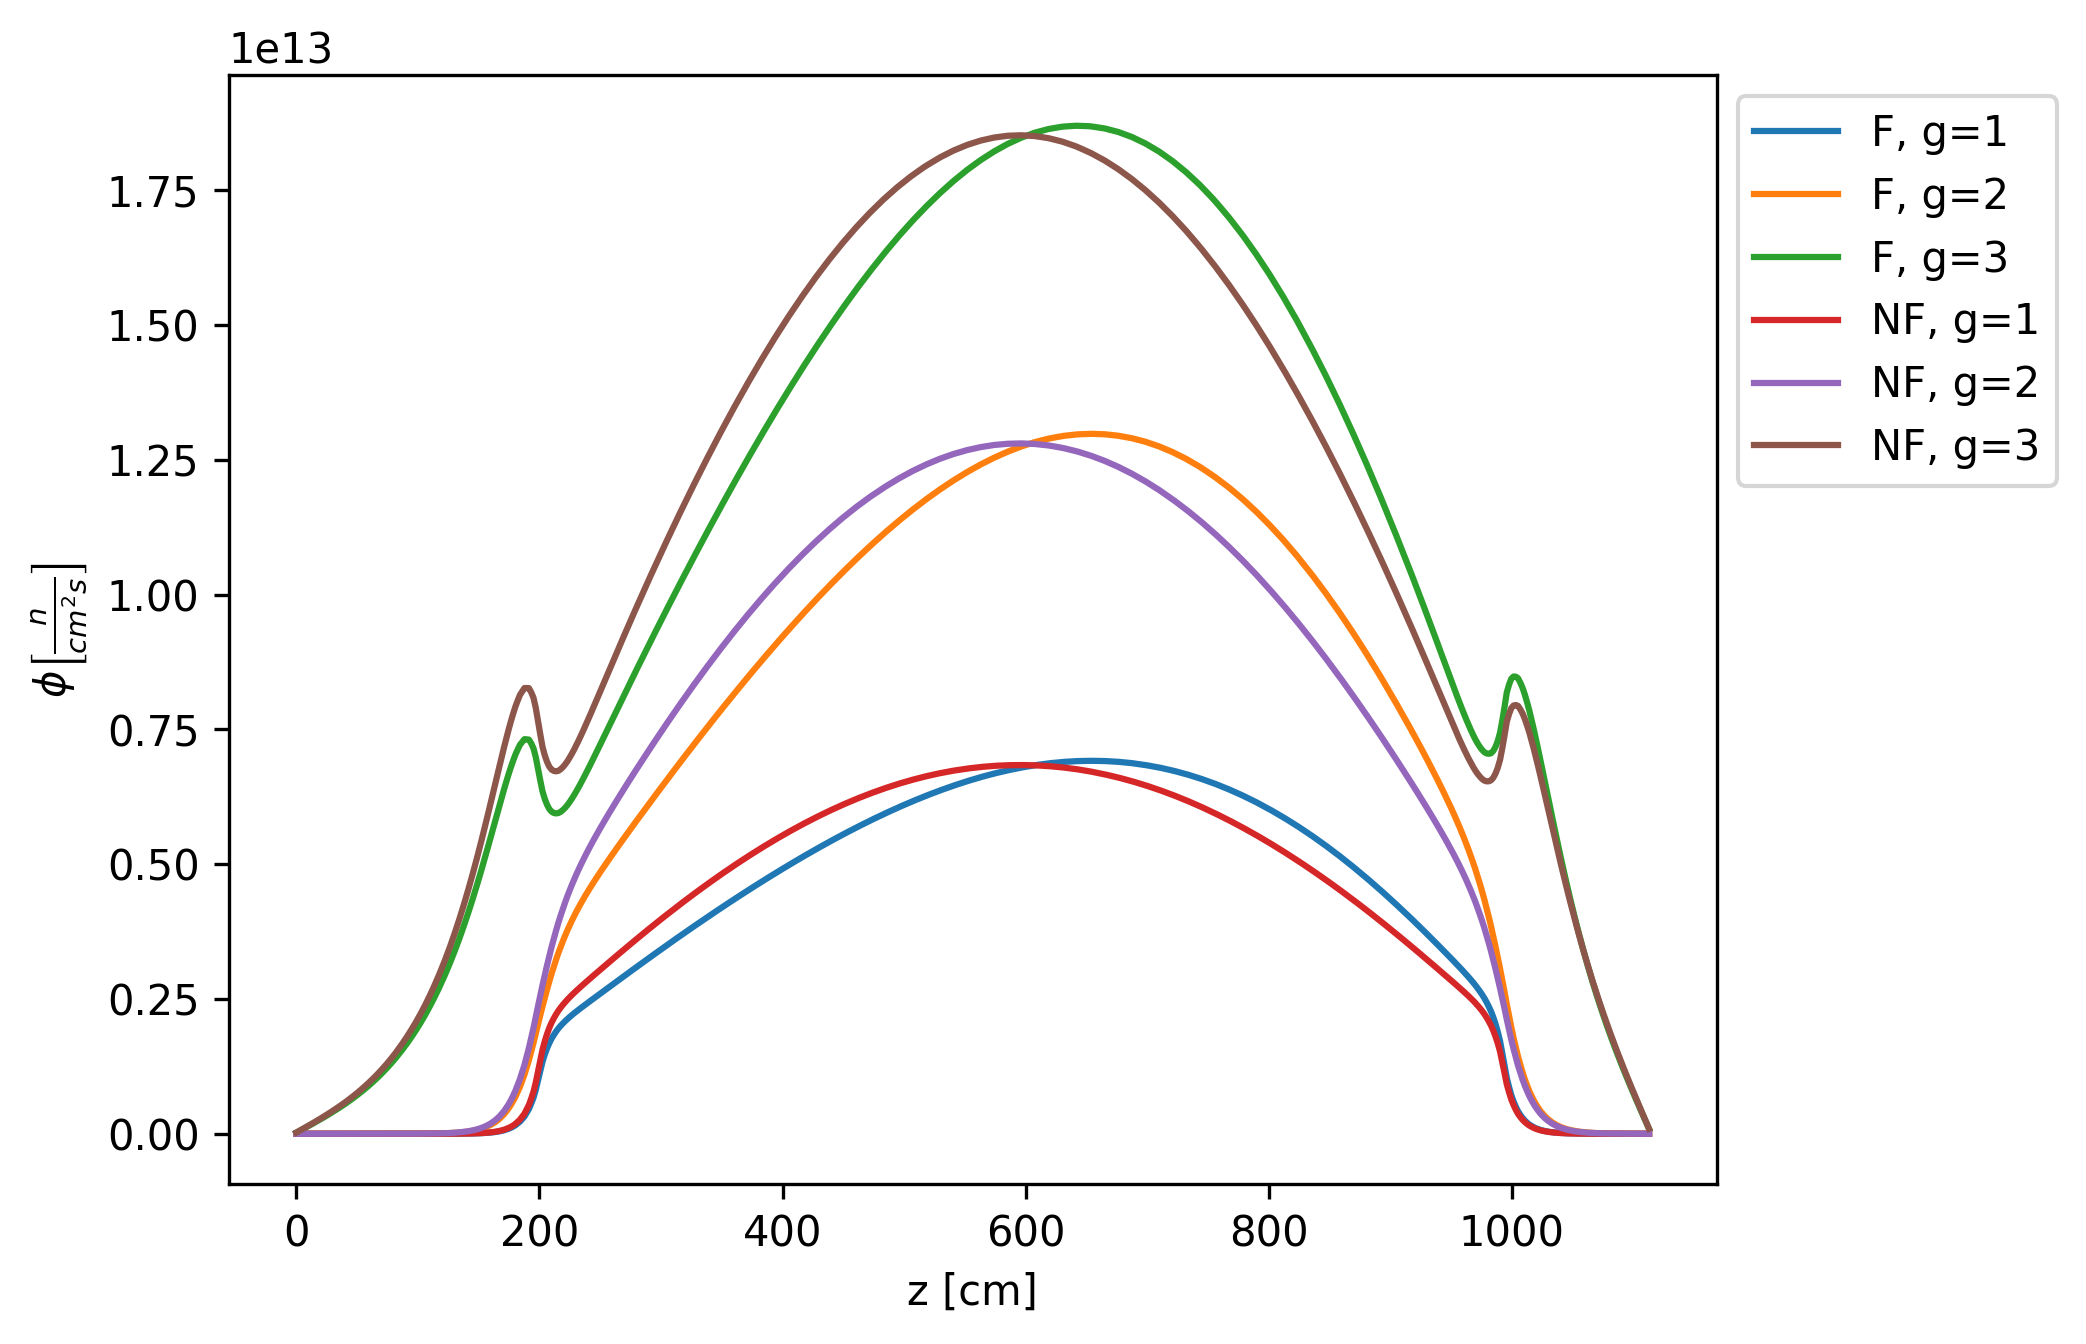
\includegraphics[width=0.45\textwidth]{figures-thermal/coupledD-3G-axial}
    }
    \subfloat[Radial temperature at z=L/2=556.5 cm]{
        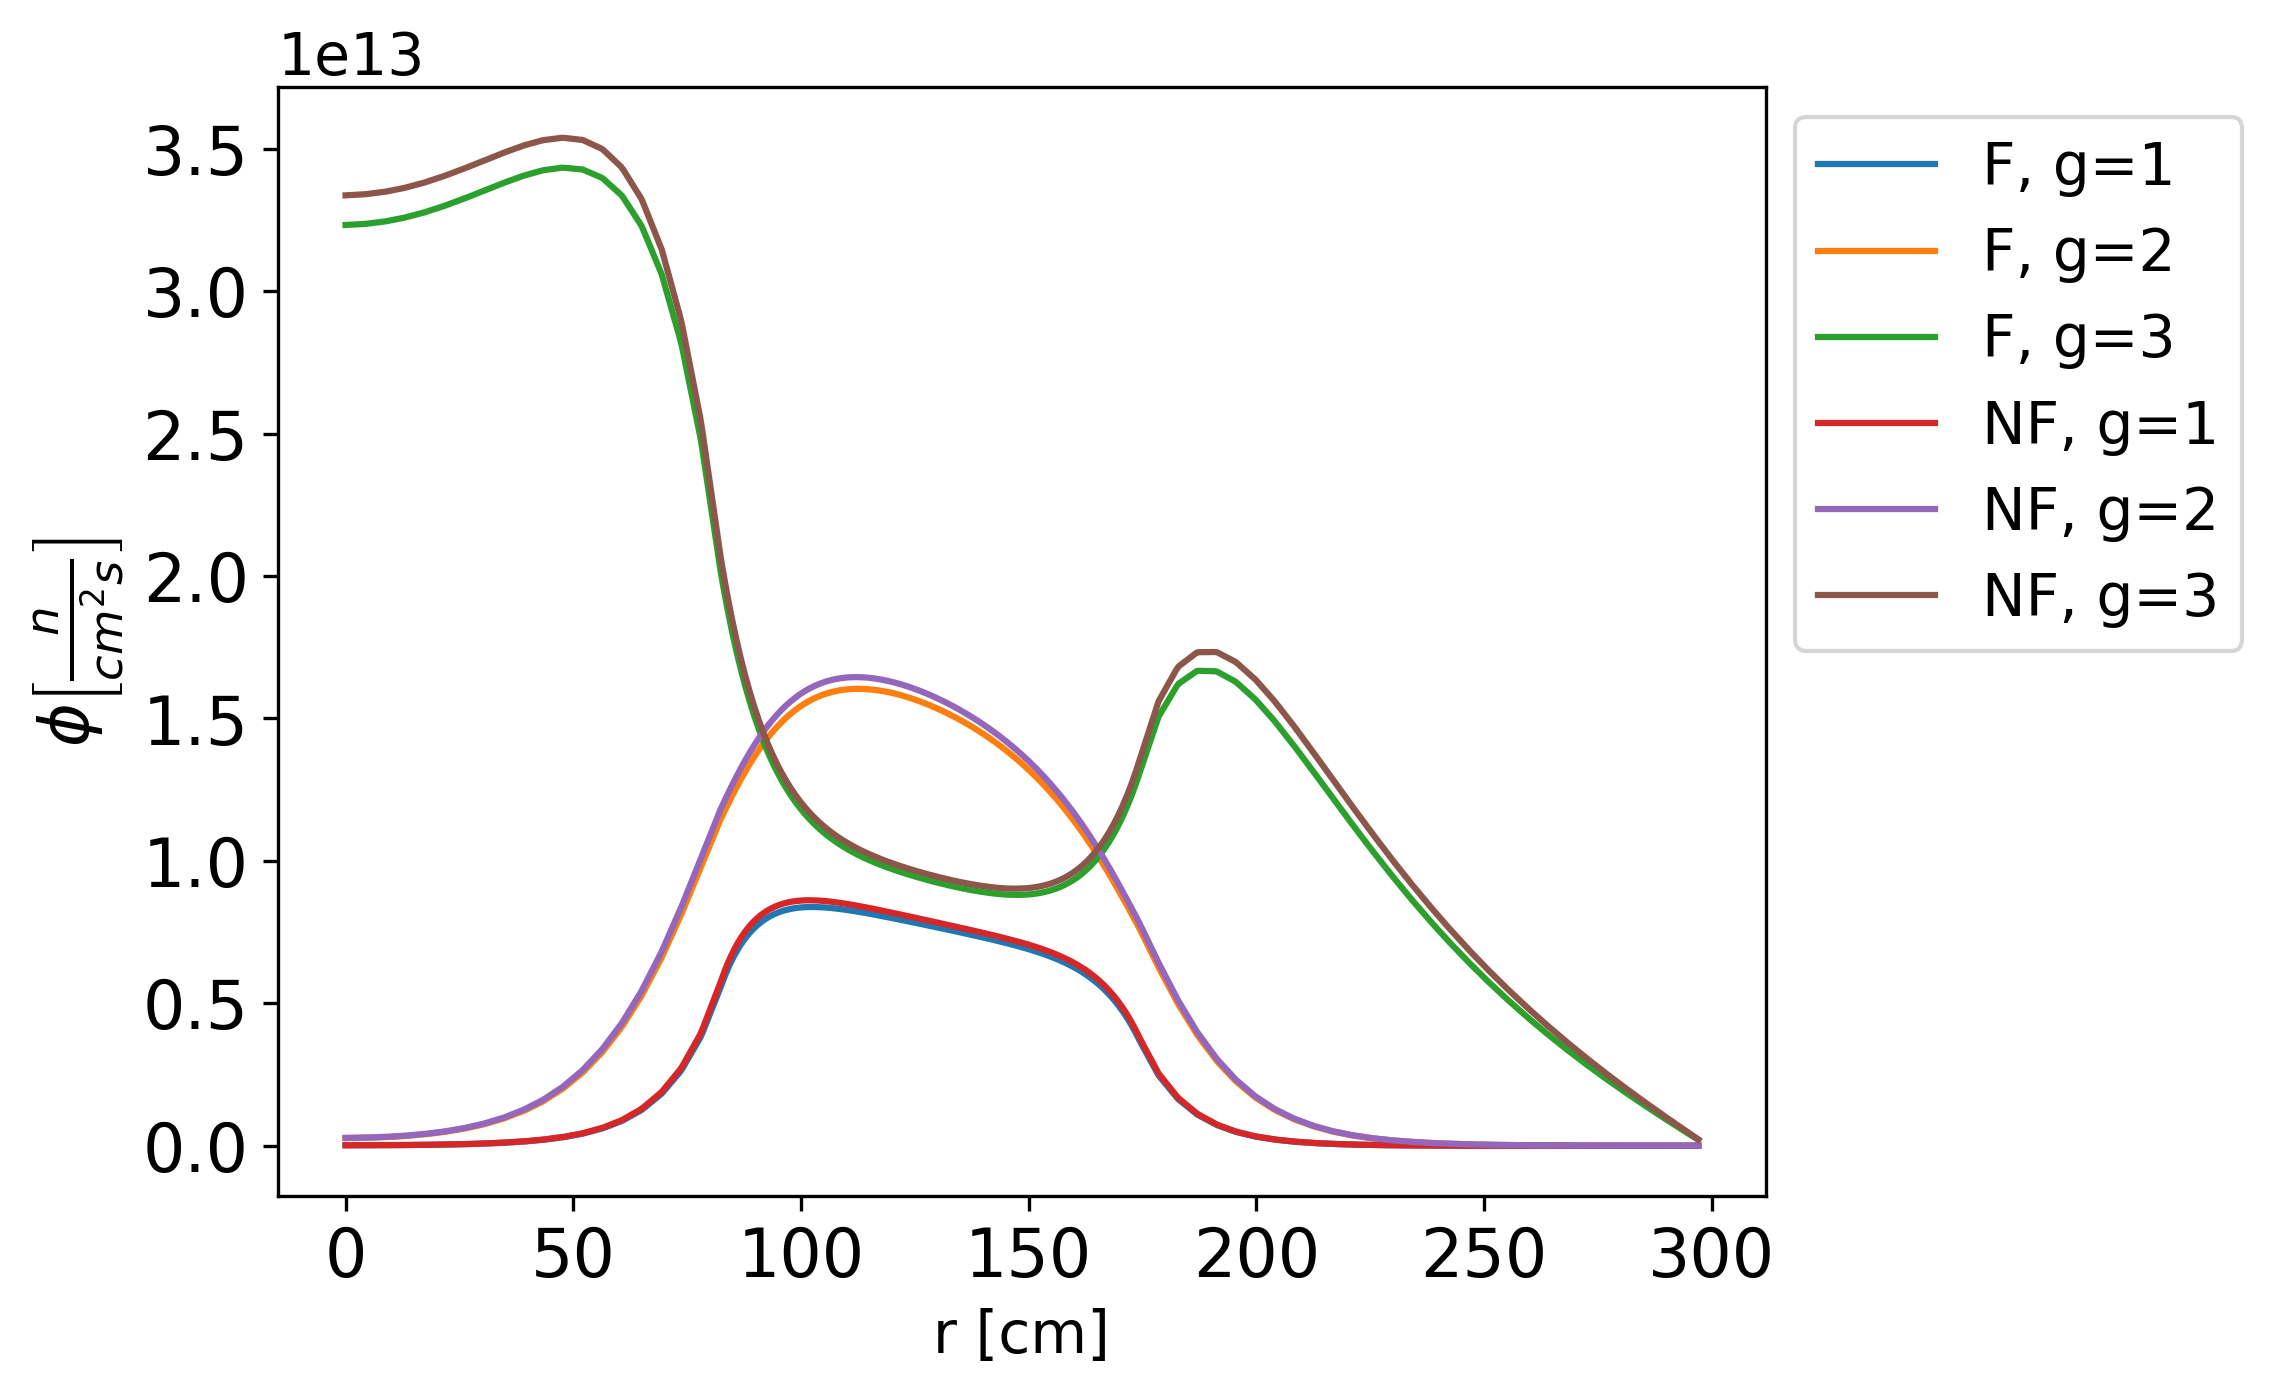
\includegraphics[width=0.45\textwidth]{figures-thermal/coupledD-3G-radial}
    }
  \hfill
  \caption{Flux profiles. F: thermal feedback, NF: no thermal feedback.}
  \label{fig:coupled-results-flux}
\end{figure}

\begin{figure}[htbp!]
  \centering
    \subfloat[Axial temperature at r=85 cm.]{
        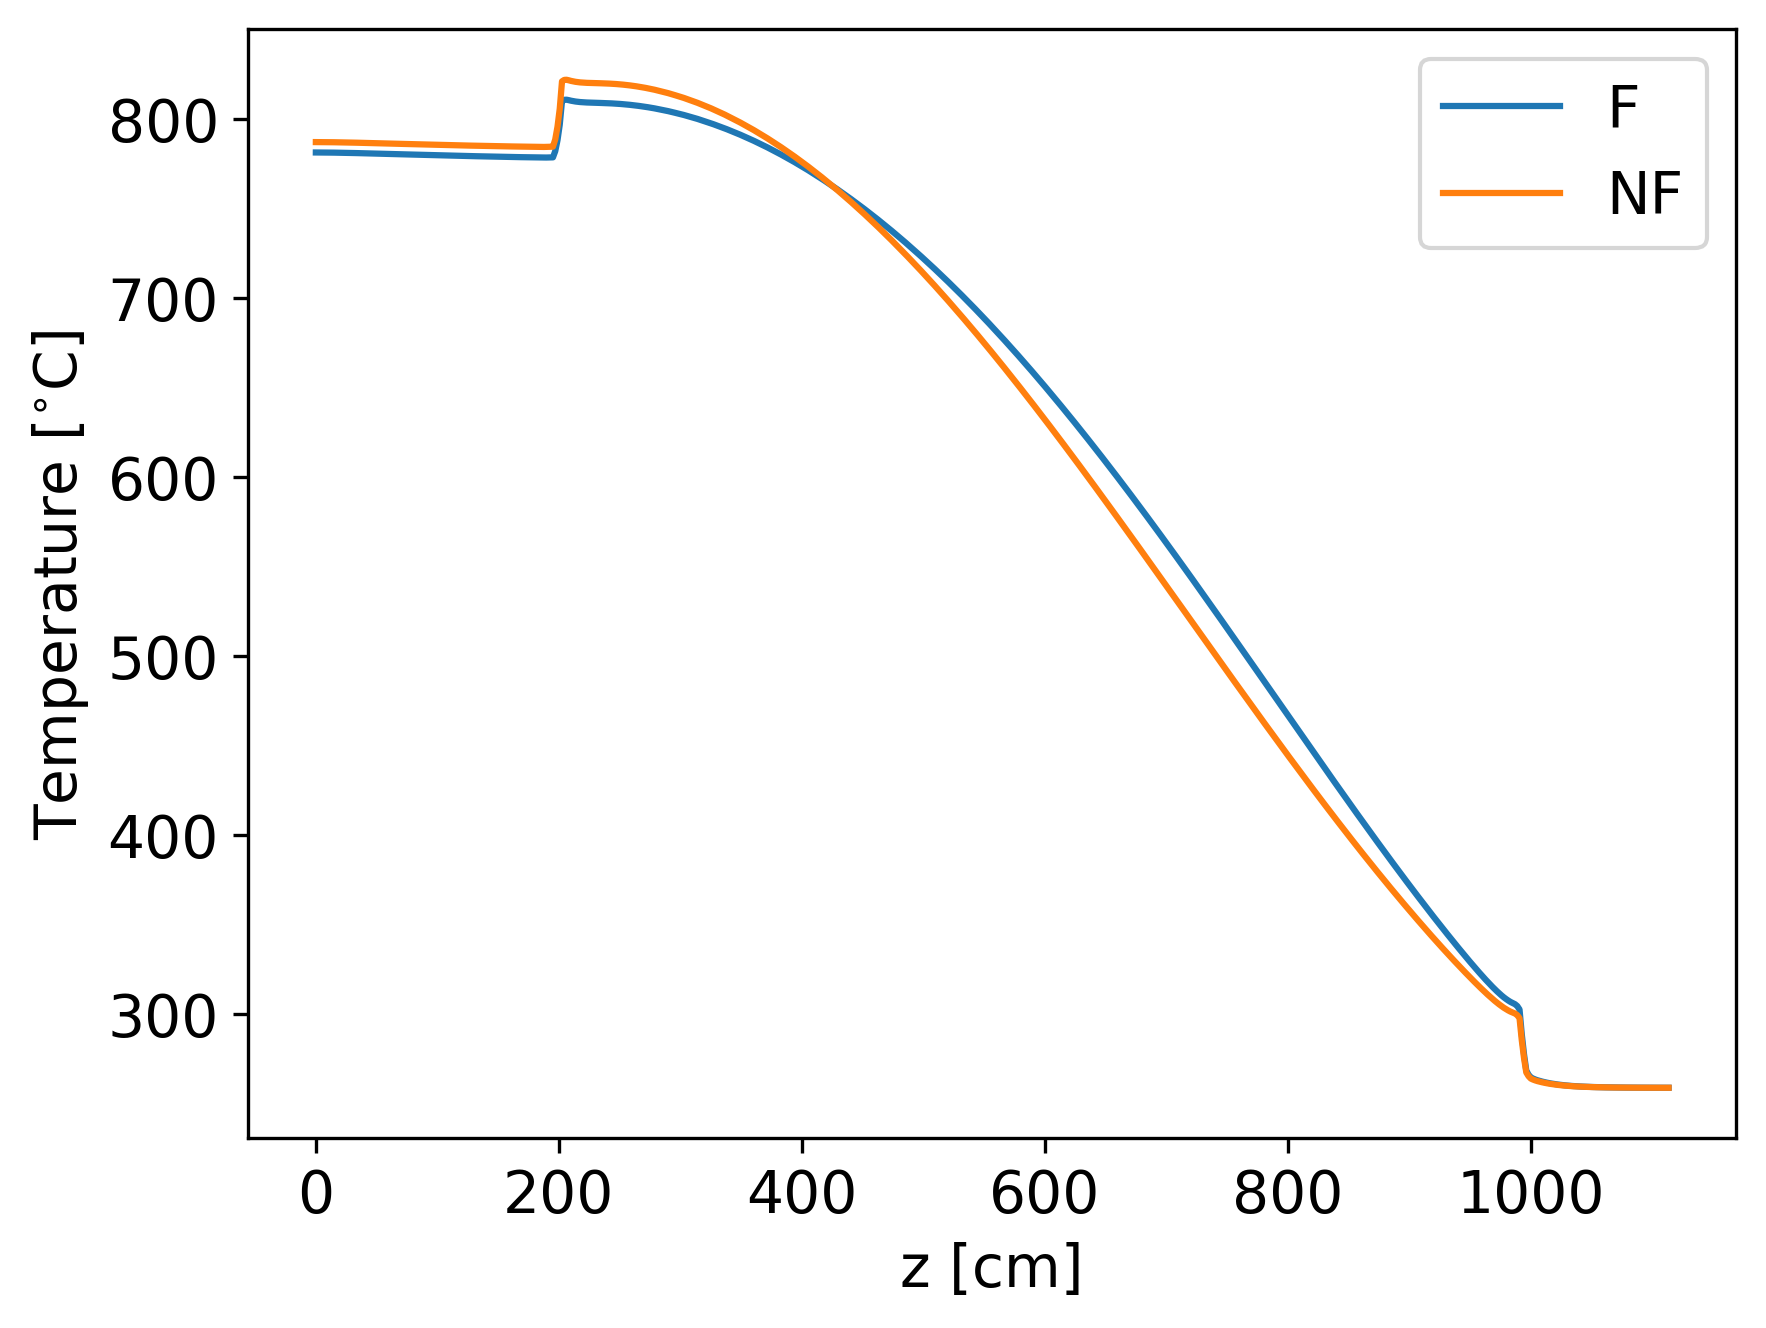
\includegraphics[width=0.45\textwidth]{figures-thermal/coupledD-3G-axialT}
    }
    \subfloat[Radial temperature at z=L/2=556.5 cm]{
        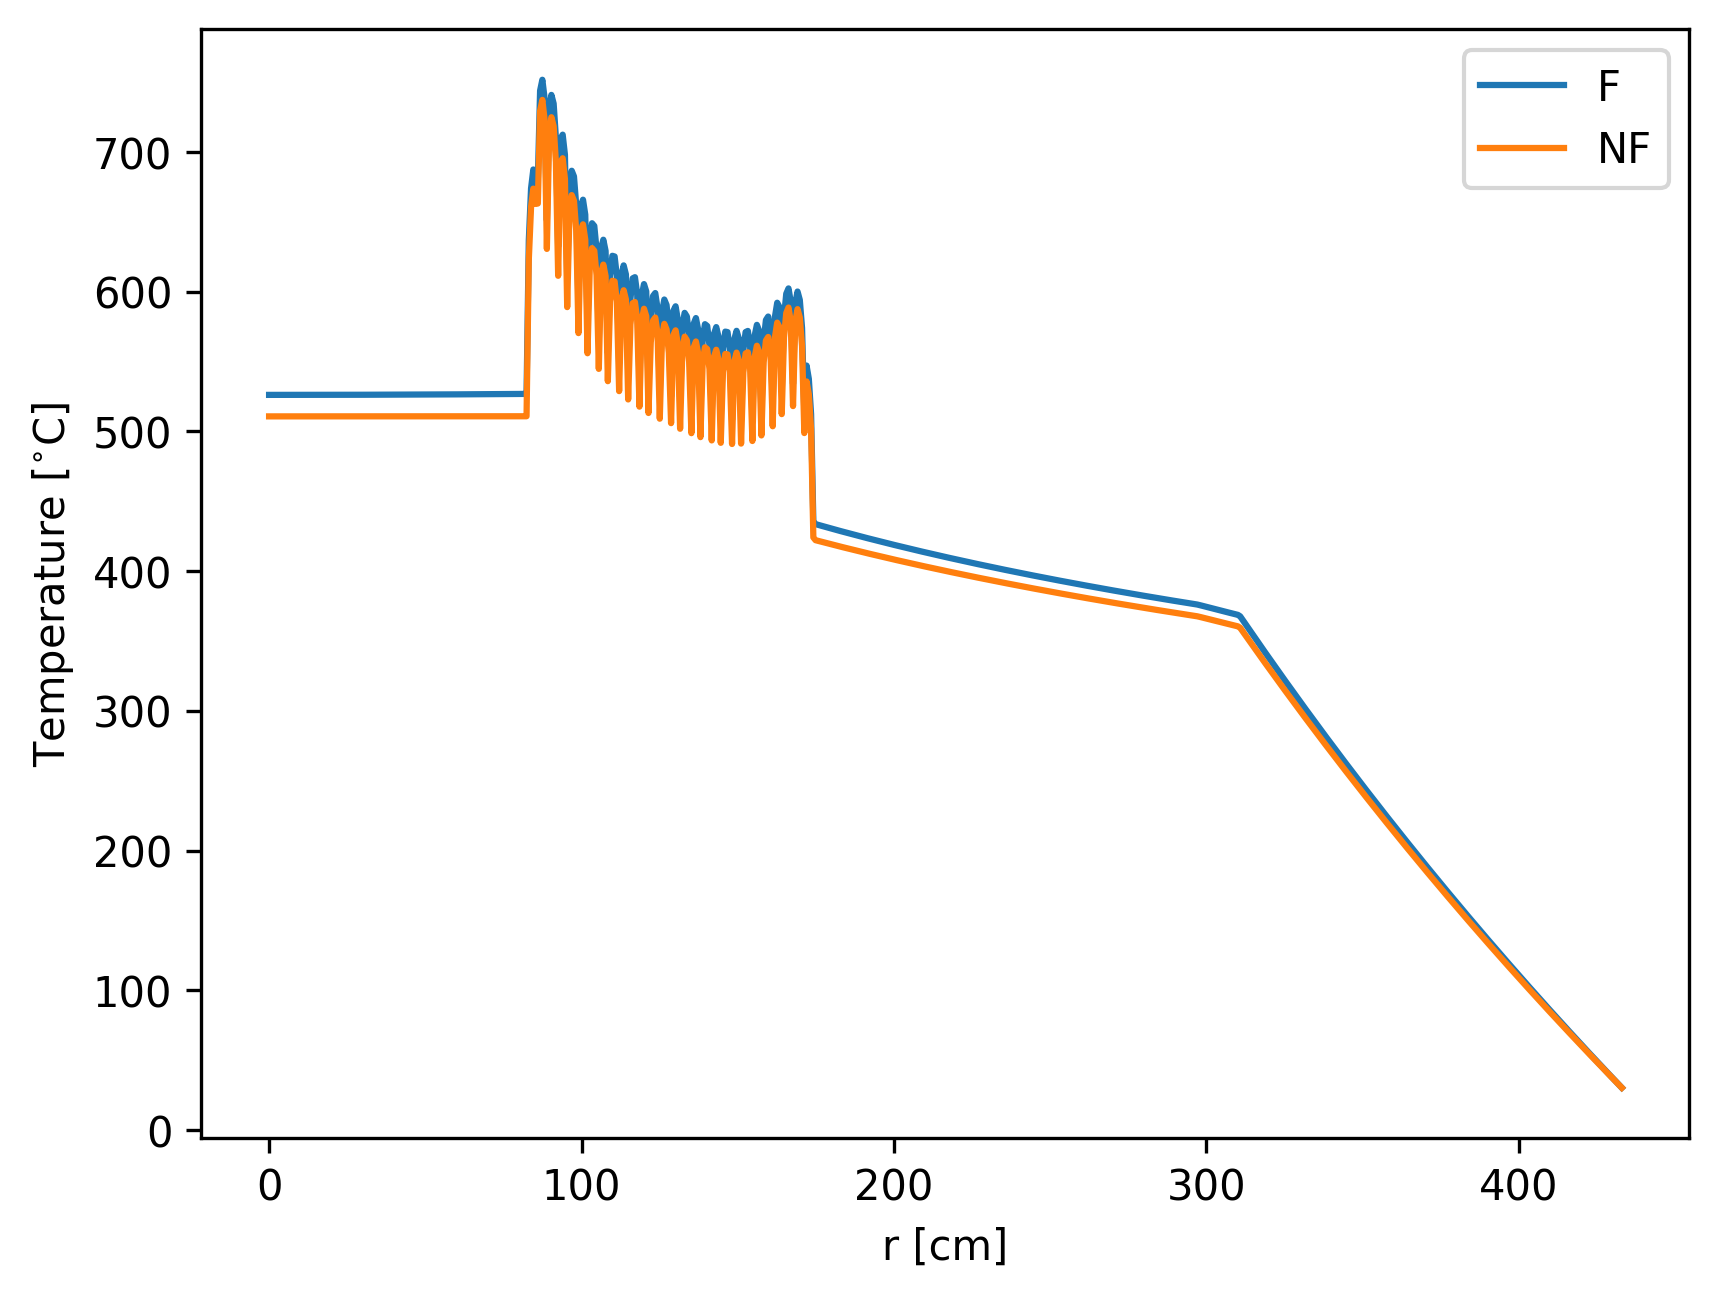
\includegraphics[width=0.45\textwidth]{figures-thermal/coupledD-3G-radialT}
    }
  \hfill
  \caption{Temperature profiles. F: thermal feedback, NF: no thermal feedback.}
  \label{fig:coupled-results-th}
\end{figure}